\chapter{Background and Notation}\label{ch:background}

This chapter introduces some mathematical formulations and definitions related to the topics discussed in this report. We start by explaining the Multi-Armed Bandits problem in section \ref{sec:mab}. 
Bayesian Optimization is introduced as continuous version of MAB in section \ref{sec:bo}. How Gaussian Processes are used as surrogate model and acquisition functions to sample the next point for evaluation is also discussed with BO. 
Then we introduce Safe Bayesian Optimization in section \ref{sec:safebo} and discussed SafeOpt algorithm, a GP based safe exploration method in section \ref{sec:safe-explore}.
A parallel Bayesian Optimization implementation is discuss in section \ref{sec:parallel-bo}, which introduces the idea of Hyperspace.

\section{Multi-Armed Bandits}\label{sec:mab}
\subsection{The Explore-Exploit Tradeoff}
The real-world decision-making process has a feature that presents uncertainty in the outcome of a future decision. So it is difficult for an agent(decision-maker) to choose the best following action due to uncertainty in the result of a given action. Most of the real-world tasks to maximize cumulative outcomes require making many sequential decisions.

Successful completion of such a task necessitates a fundamental tension: a decision-maker (agent) must constantly choose between exploiting all known good possibilities and researching unknown but potentially better options. This conflict is known as the explore-exploit tradeoff, and it is the basis for improving decision-making.

The explore-exploit tradeoff is observed in various natural and artificial systems. Foraging animals in the natural world strive to consume as much food as possible while also seeking out the most rewarding foraging areas \cite{Keasar:2002}.

\subsection{Multi-Armed Bandit Problem}
\hspace*{0.7cm}The Multi-armed Bandit (MAB) problem is a classic mathematical description of the explore-exploit tradeoff \cite{Robbins:1952}. 
A decision-maker(agent) is faced with a sequential series of decisions in the MAB problem. Each choice requires the decision-maker(agent) to pick between two or more options, often known as arms, each of which has a probability distribution associated with it that models the reward. 
The decision-maker receives a noisy reward chosen from the related probability distribution after selecting an option. The goal of the decision-maker is to maximise their expected cumulative reward, which is comparable to selecting the option with the highest mean as often as possible.

\subsubsection{Model and Example}
We consider\textcolor{white}{"}the basic model with \textit{IID} rewards, called \textit{stochastic  bandits} \cite{mab-intro}. An algorithm has $K$ possible actions to choose from, a.k.a. \textit{arms}, and there are $T$ rounds, for some known $K$ and $T$ . In each round, the algorithm chooses an arm and collects a reward for this arm. The algorithm’s goal is to maximize its total reward over the $T$ rounds. We are primarily interested in the mean reward vector $\mu \in [0, 1]^K$, where $\mu(a) = \mathbb{E}[\mathcal{D}_a]$ is the mean reward of arm $a$.\textcolor{white}{"}

\begin{algorithm}[H]
%	\SetAlgoVlined
	\caption{\texttt{Epsilon-greedy algorithm}}
	\For{$each\ round\ t \in T$}
	{
		toss a coin with success probability $\epsilon$;\\
		\eIf{success}
		{
			explore: choose an arm uniformly at random
		}
		{
			exploit: choose the arm with the highest average reward so far
		}
	}
\end{algorithm}
Some motivating examples,\\
\textbf{Ad selection}: In website\textcolor{white}{"}advertising, a user visits a webpage, and a learning algorithm selects one of many possible ads to display. If ad $a$ is displayed, the website observes whether the user clicks on the ad, in which case the advertiser pays some amount $v_a \in [0, 1]$. So each ad is an arm, and the paid amount is the reward.\\
\textbf{Medical Trials}: a patient visits a doctor and the doctor can prescribe one of several possible treatments, and observes the treatment effectiveness. Then the next patient arrives, and so forth.\textcolor{white}{"}
\begin{definition}
	For best arm $\mu^*$ and total rounds $T$, the difference between cumulative reward to the \textit{best-arm benchmark} $\mu^* \cdot T$ is called \textit{regret} at round $T$:
	$$ \mathbb{E}\left[ R(T)\right]  = \mu^* \cdot T - \mathbb{E} \left[ \sum_{t=1}^{T}\mu(a_t) \right] $$
\end{definition}
Since $R(T)$ is a random variable, so the \textit{expected} regret.
%$\mathbb{E}[R(T)]$.

\section{Bayesian Optimization}\label{sec:bo}
We want to optimize a function $f : \mathcal{X} \to \mathbb{R}$ over some set $\mathcal{X}$ (here the set $\mathcal{X}$ is the set of hyperparameters we want to search over). But $f$ is expensive to compute and the gradients are also not available, thus making optimization difficult.,\textcolor{white}{"}making optimization difficult\cite{cs4787}. Main idea of Bayesian optimization:\textcolor{white}{"}
\begin{itemize}
	\item Model $f$ as\textcolor{white}{"}a probability distribution.\textcolor{white}{"}
	\item If we’ve computed $f$ at parameter values $x_1, x_2, \dots , x_D$, then we consider\\ $f (x_1), f(x_2), \dots , f(x_D)$ to be \textit{observed variables} in the model.
	\item Any $x$ that we haven’t computed $f(x)$ for corresponds to a \textit{unobserved variable} in the model.
	\item Fundamental approach is, though $f(x)$ is not evaluated, we can get the conditional distribution  $ P(f(x)|f(x_1), f(x_2), \dots , f(x_D))$ from defined probabilistic model. The choice of probabilistic model should be such that, it is much cheaper to compute than origional function $f(x)$ itself.
	\item We\textcolor{white}{"}can use this conditional distribution to estimate $f(x)$ for values of $x$ we haven’t observed yet.\textcolor{white}{"}
	\item The conditional distribution helps us chose next value of $x$ at which we evaluate $f(x)$. We obtain a sequence of $f(x)$ which is used for future optimization process.
	\item The involvement of previous evaluations are beneficial for better optimization. Such a strategy is in the core of the Bayesian Optimization process. This method is in accordance with other methods like Gradient Descent and Momentum.
\end{itemize}
Two major design decisions for Bayesian optimization:
\begin{itemize}
	\item \textbf{Prior}: The prior captures the belief of the objective function. Use of wrong priors can lead to wrong follow up in the modelling. A very elegant solution exists to address this problem which is known as applying a Gaussian Process based prior.
	\item \textbf{Acquisition function}: How\textcolor{white}{"}we select the next point to sample, given a conditional distribution over the values of $f(x)$.\textcolor{white}{"} 
\end{itemize}

\subsection{Gaussian Processes}
A GP is an infinite-dimension stochastic process that extends the multivariate Gaussian distribution to any finite combination of dimensions. \cite{Freitas-BO}. A GP is a distribution over functions that are totally characterized by its mean function $m$ and covariance function $k$, just like a Gaussian distribution is a distribution over a random variable that is completely specified by its mean and covariance: 
$$ f(x) \sim \mathcal{GP}(m(x),k(x,x^\prime)) $$
It is\textcolor{white}{"}often valuable to intuitively think of a GP as analogous to a function. However, instead of returning a scalar $f(x)$ for an arbitrary $x$, it returns the mean and variance of a normal distribution over (see fig.\ref{fig:gp-example}) the possible values of $f$ at $x$. 
In figure \ref{fig:gp-example}, for three observations, with a simple 1D Gaussian process used. The shaded region displays the mean plus and minus the variance, while the solid black line is the GP surrogate mean forecast of the objective function given the data. At the coordinates $x_{1:3}$, the overlaid Gaussians correspond to the GP mean and standard deviation ($\mu(\cdot)$ and $\sigma(\cdot)$) of prediction.
Stochastic processes are sometimes called \textit{random functions} by analogy to random variables.\textcolor{white}{"}
\begin{figure}[H]
	\centering
	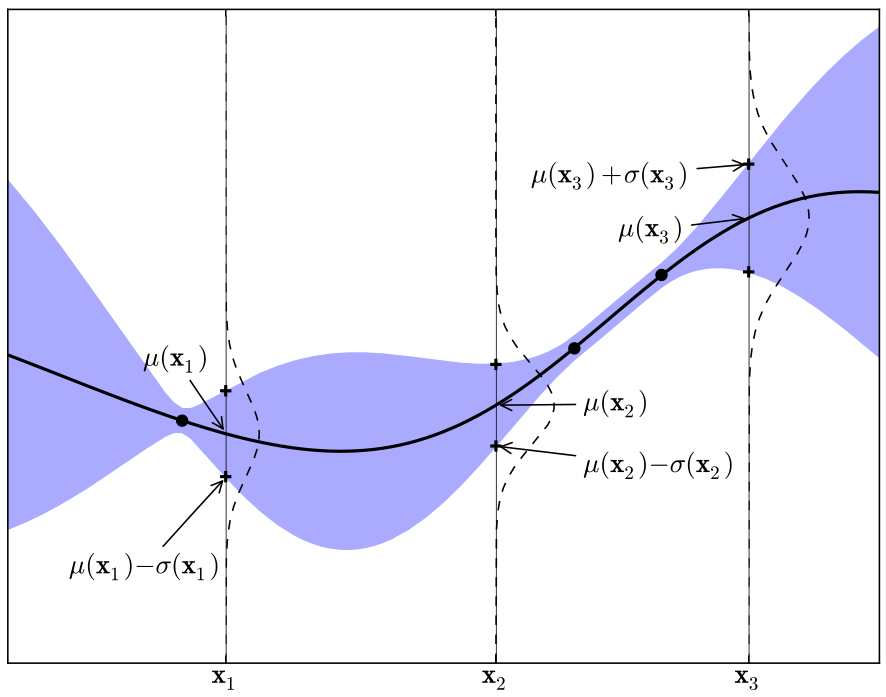
\includegraphics[scale=0.40]{figures/gp.png}
	\caption{Gaussian Processes regression.}
	\label{fig:gp-example}
\end{figure}

% include regarding kernels
% explain aquisition functions
\subsection{Acquisition Functions}
Acquisition functions help us sample new points from the domain $x \in X$. The acquisition function uses tools of probability and statistics to arrive at the new point to be sampled. It acts as a guide for the parameter space to explore during Bayesian Optimization.\\
Some widely used acquisition functions are,
\begin{itemize}
	\item Probability of improvement
	\item Expected improvement
	\item Upper confidence bound
\end{itemize}

\section{Safe Bayesian Optimization}\label{sec:safebo}
In safe Bayesian optimization, instead of optimizing the unknown objective function $f(x)$ globally, it finds the maximizer within the safe set defined by safety constraints that are unknown to the agent. 
So, this safe set is not known initially, but estimated after each safety constraints evaluation. So it is a technique, focused on solving the problem
$$ \max_{x_t\in\mathcal{X}}\text{ such that }g(x_t)\geq 0, \forall t\text{ with probability }\geq 1-\delta $$
\begin{figure}[H]
	\centering
	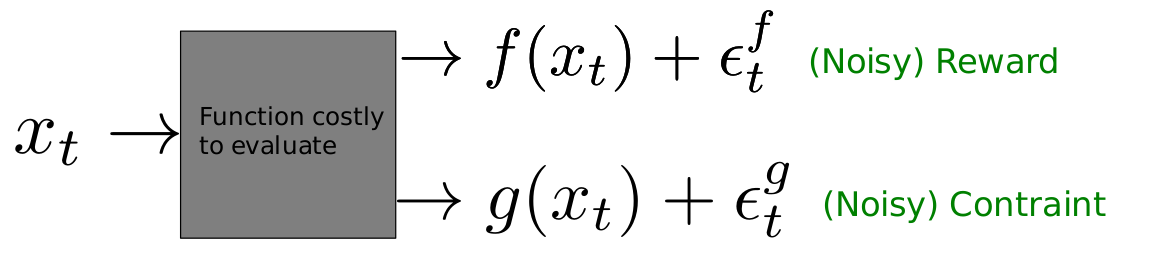
\includegraphics[scale=0.30]{figures/safebo.png}
	\caption{Safe Bayesian optimization illustration}
	\label{fig:safebo}
\end{figure}

The formal problem setting of the safe Bayesian optimization can be explained by figure \ref{fig:safebo} (only one safety constraint is considered, could be multiple). So at time $t$ agent selects an action $x_t$ from the estimated safe set (every $x$ in the estimated safe set should satisfy the safety constrain with high probability) and interact with the environment and observe the noisy observations $y_t$ and $z_t$ of the objective function $f(\cdot)$ and safety function $g(\cdot)$ at $x_t$ respectively. Furthermore, add $(x_t, y_t, z_t )$ to the buffer or train set from which it updates the Bayesian belief about the unknown objective and safety function.

\section{GP based Safe Exploration Algorithms}\label{sec:safe-explore}
A GP is well suited for safety-critical problem settings. The unknown safety functions are modeled using GP, and the uncertainty of these functions is given by the confidence interval (i.e., variance) of their respective GPs. The confidence interval is used to take a safe action with high probability. The following section will explain the SAFEOPT (safe exploration in a Bandit or stateless setting).

\subsection{SafeOpt}
To guarantee safety in bandit setting problems Sui et al.\cite{sui15} proposed \texttt{SafeOpt} algorithm. The objective is to optimize an unknown function f (x) subject to safety constraints.
For that, they have used a safe Bayesian optimization framework (see section \ref{sec:safebo}). 
In their setting they considered the safety as, for chosen action/parameter $x_t$ at time $t$ the function value $f(x_t)$ should greater than a safety threshold $h$. 
As a result, the authors use Gaussian process (GP) regression to solve the problem of predicting the maximum of an unknown function $f(x)$. 
The unknown function is considered to be represented by a sample function from a GP prior in GP regression \cite{RasmussenW06}.
The GP prior is fully defined by its mean function $\mu(x)$ (with no loss of generality, $\mu(x) = 0$) and covariance function $k(x, x^\prime )$, where $x, x^\prime \in \mathcal{X}$.
%Thus the authors approach the problem of estimating the maximum of the unknown function $f(x)$ by estimating $f(x)$ using Gaussian process (GP) regression. 
%In GP regression, the unknown function is assumed to be modeled by a sample function from a GP prior \cite{RasmussenW06}. 
%The GP prior is completely characterized by its mean function $\mu(x)$ (without loss of generality $\mu(x) = 0$) and covariance function $k(x, x^\prime )$ where $x, x^\prime \in \mathcal{X}$. 
At every time $t$, the SafeOpt\textcolor{white}{i}policy\textcolor{white}{i}chooses a\textcolor{white}{i}point $x_t$ and\textcolor{white}{i}receives an\textcolor{white}{i}observation $y_t = f (x_t) + n_t$ where $n_t$ is an\textcolor{white}{i}independent sample from\textcolor{white}{i}Gaussian noise with\textcolor{white}{i}mean 0 and\textcolor{white}{i}variance $\sigma^2$. 
A posterior distribution for the unknown function may be calculated using $y_t$.
This posterior distribution is again Gaussian, with a mean function $\mu_t(x)$ and a covariance function $k_t (x, x^\prime)$ that characterise it perfectly.
%Based on $y_t$, a posterior distribution for the unknown function can be derived. 
%This posterior distribution is again Gaussian and characterized completely by a mean function $\mu_t(x)$ and covariance function $k_t (x, x^\prime)$. 
SafeOpt uses this posterior to compute upper and lower confidence bounds on the function in order to meet the safety criteria. 
%In order to satisfy the safety constraints, SafeOpt computes upper and lower confidence bounds on the function using this posterior. 
The\textcolor{white}{i}upper $u_t(x)$ and\textcolor{white}{i}lower $l_t(x)$ confidence\textcolor{white}{i}bounds are defined as 
$$u_t(x)=\mu_t(x)+\beta_t\sigma_t(x),$$
$$l_t(x)=\mu_t(x)-\beta_t\sigma_t(x).$$
And it uses the confidence interval $Q_t(x) = [l_t(x), u_t(x)]$ to estimate a safe set $S_t\subset \mathcal{X}$, from which agent select a next query point $x_{t+1}$ for which the function value $f(x_{t+1})$ is greater than safety threshold with high probability. 
Safe Set $S_t$ is defined as:
$$ S_t \gets \cup_{x\in S_{t-1}}\{ x^\prime \in \mathcal{X} | l_t(x) - Ld(x,x^\prime) \geq h \} $$
where $L$ is lipschitz constant. 
SafeOpt assume at $t = 0$ it is provided with a initial safe seed $S_0$. 
SafeOpt\textcolor{white}{i}keeps track of a set $G_t \subseteq S_t$ of candidate\textcolor{white}{i}decisions that, if chosen again, have the\textcolor{white}{i}potential to\textcolor{white}{i}expand $S_t$.
%SafeOpt maintains a set $G_t \subseteq S_t$ of candidate decisions that, upon potentially repeated selection, have a chance to expand $S_t$. 
The set $G_t$ is defined as
$$ G_t = \{x \in S_t | \psi_t(x) > 0 \} $$
where
$$ \psi_t(x) = |\{ x^\prime \in \mathcal{X} \backslash S_t | u_t(x) - Ld(x,x^\prime) \geq h \}| $$
To\textcolor{white}{i}discover the maximum, SafeOpt\textcolor{white}{i}keeps a separate set of $M_t \subseteq S_t$ decisions\textcolor{white}{i}that are possible $f$ maximizers.
%In order to find the maxima SafeOpt maintain a another set $M_t \subseteq S_t$ of decisions that are potential maximizers of $f$.
$$ M_t = \{ x \in S_t |u_t(x) \geq \max_{x^\prime \in S_t} l_t(x^\prime) \} $$
SafeOpt\textcolor{white}{i}policy then chooses points $x_t$ according\textcolor{white}{i}to $$ x_t = \argmax_{x\in G_t \cup M_t}w_t(x) $$
where $w_t(x)=u_t(x)-l_t(x)$.

The pseudo-code for the SafeOpt algorithm is given below. For a high-level description of the SafeOpt, please refer to Sui et al. paper \cite{sui15}.\\

\begin{algorithm}[H]
	\caption{\texttt{SafeOpt}}
	\label{alg:safeopt}
	\KwIn{Function\textcolor{white}{i}domain $\mathcal{X}$ , GP\textcolor{white}{i}prior $(\mu, k)$, signal variance\textcolor{white}{i}parameter $\sigma_0$ , seed\textcolor{white}{i}set $S_0$, safety\textcolor{white}{i}threshold $h$, Lipschitz\textcolor{white}{i}constant $L$.}
	$C_0(x) \gets [h, \infty), \forall x \in S_0$\\
	$C_0(x) \gets \mathbb{R}, \forall x \in \mathcal{X} - S_0$\\
	$Q_0(x) \gets \mathbb{R}, \forall x \in \mathcal{X}$\\
	\For{$t=1,\dots$}
	{
		$C_t(x) \gets C_{t-1}(x) \cap Q_{t-1}(x)$\\
		$S_t \gets \cup_{x\in S_{t-1}}\{ x^\prime \in \mathcal{X} | l_t(x) - Ld(x,x^\prime) \geq h \}$\\
		$G_t = \{x \in S_t | \psi_t(x) > 0 \}$\\
		$M_t = \{ x \in S_t |u_t(x) \geq \max_{x^\prime \in S_t} l_t(x^\prime) \}$\\
		$x_t = \argmax_{x\in G_t \cup M_t}w_t(x)$\\
		$y_t = f(x_t)+n_t$\\
		Compute $Q_t(x), \forall x \in S_t$\\
		if $\max_{ x\in G_t \cup M_t}w_t(x) \leq \epsilon$ then Break
	}
\end{algorithm}

\section{Parallel Bayesian Optimization}\label{sec:parallel-bo}
Some ML models such\textcolor{white}{"}as non-negative matrix factorization (NMF) have relatively few hyperparameters. 
However, emerging deep learning (DL) algorithms often consist of significantly more tunable parameters. 
As the number of model hyperparameters increases, their optimization becomes significantly more challenging as we face a combinatorial increase in potential model configurations. 
Similarly, there is an increased chance that our models' hyperparameters interact in complex ways. 
Modeling these interactions in high-dimensional search spaces quickly becomes challenging and can often defy our intuition. 
Even experts find it difficult to manually configure hyperparameters.

So, parallel optimization leverages high performance computing (HPC) resources to better understand unknown, potentially non-convex hyperparameter search spaces.\textcolor{white}{"}

\subsection{Hyperspace}
\texttt{HyperSpace}\cite{YoungHRK18} approaches\textcolor{white}{"}parallelism by concurrently running many Gaussian processes over our large hyperparameter search space. 
This is done by partitioning the hyperparameter search space, allowing us to model many regions of potential algorithm configurations. 
Authors emphasize the partitioning the search space since we are interested in how the changes of this optimization space affects our learner’s performance. 
This differs from the parallel approach presented in \cite{SnoekLA12}, where the authors parallelize a single Gaussian process. 
By running many GPs in parallel, we are able to compare our models' performance over various areas in the large hyperparameter search space as each GP grants a unique perspective over the
space. 
More critically, partitioning the search space means that a more detailed search is performed as many more models are explored across a diverse set of search spaces.

This addresses concerns of exponential scaling acknowledged in early papers on Bayesian optimization theory \cite{pmlr-v9-grunewalder10a} \cite{Srinivas.2012}, which showed that as number of search dimensions increase, Bayesian optimization requires many more queries of the objective function in order to bound our uncertainty about the optimization process, thus increasing the odds of finding near optimal values.\textcolor{white}{"}

\subsubsection{Creating HyperSpaces}
The hyperparameter search space is divided as follows.
\begin{itemize}
	\item For each hyperparameter, define a lower and an upper bound.
	\item Then divide each hyperparameter bound into two near equally sized subspaces with a degree of overlap, $ \phi \in [0,1] $.
	\item When $\phi=0$, there is no overlap between the subspaces.
	\item When $\phi=1$, there is perfect overlap, and two copies of the original space are created.
	\item After dividing the original search space, create all possible combinations of these subintervals, called \textit{hyperspaces}.
\end{itemize}
A total of $2^H-S$ subspaces\textcolor{white}{"}are created where $H$ is the number of hyperparameters whose interval bounds exceed some minimal length, $\alpha$, and $S$ is the number of hyperparameters whose interval bounds length is less than $\alpha$.
These hyperspaces are subsequently distributed across an HPC(High-Performance Computing) system.
Then run the Bayesian optimization loop for some predetermined $m$ iterations in parallel at each node.\textcolor{white}{"}\\

\begin{algorithm}[H] 
	\caption{\texttt{HyperSpace}}
	\KwIn{Hyperparameter intervals, minimal subinterval length $\alpha$, overlap $\phi$.}
	\KwOut{Optimization results over $2^N$ hyperspaces}
	\ForEach{hyperparameter interval}
	{
		\eIf{interval length $\geq \alpha$}
		{
			divide interval into two nearly equal subintervals with overlap $\phi$;
		}
		{
			do not split;
		}
	}
	combine all possible subintervals to form hyperspaces;\\
	\ForEach{hyperspace}
	{
		run Bayesian optimization;
	}
	\Return optimization results for each hyperspace
\end{algorithm}
\vspace{2em}
By leveraging HPC resources, HyperSpace\textcolor{white}{"}can run $(2^H-S) * m$ iterations of Bayesian optimization when it takes traditional SMBO algorithms to run $m$ iterations.

Figure \ref{fig:hspex} shows partitioning two hyperparameters with HyperSpace. Two hyperparameters, both integer-valued, are each represented as a vector of eight elements. 
Each hyperparameter is divided into two equal subintervals consisting of four elements. 
For $\phi = 0.25$, a single element from the lower and upper subintervals are appended to each subinterval, respectively, making each subinterval of size five. The lower subinterval's maximum is now the minimum of the upper subinterval and vice versa. 
Finally, all possible hyperparameter subintervals are combined to create the distributed search spaces of HyperSpace.\textcolor{white}{"}


\begin{figure}[H]
	\centering
	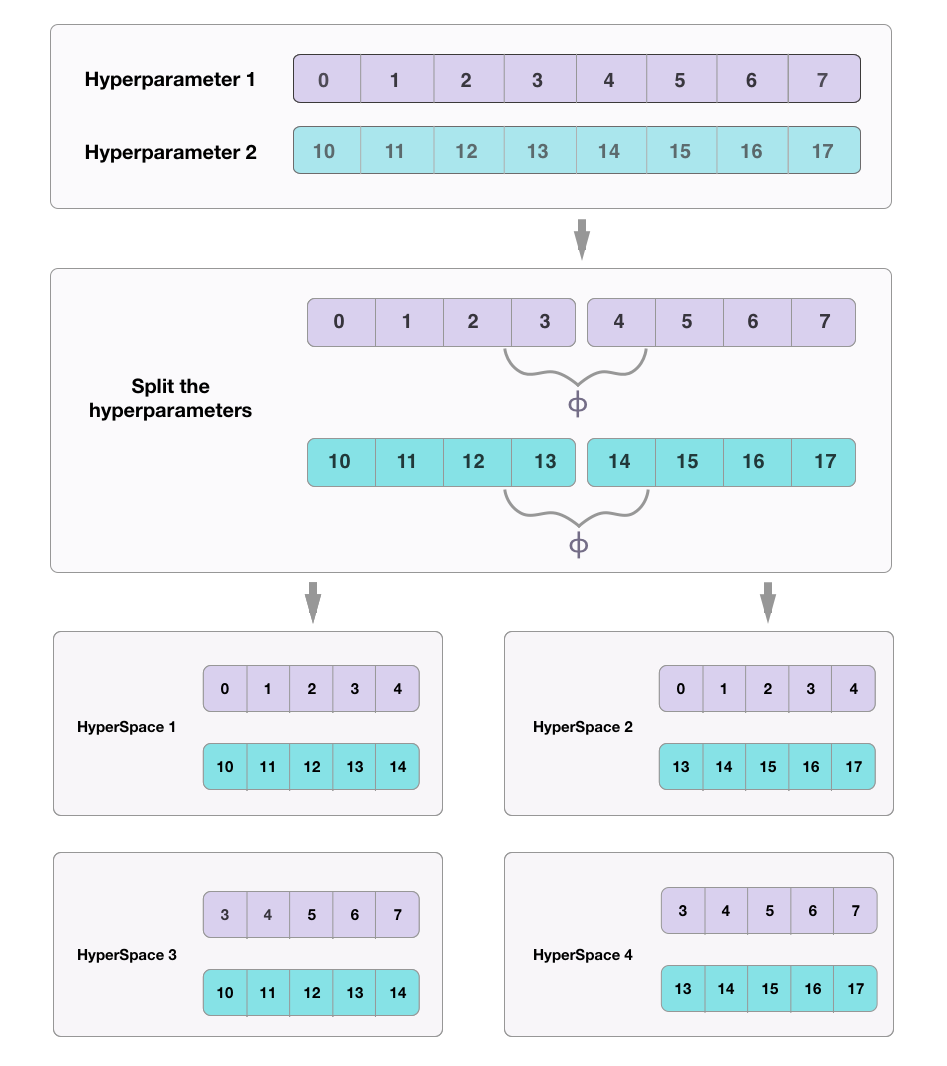
\includegraphics[scale=0.43]{figures/hyperspace-example.png}
	\caption{Partitioning two hyperparameters with HyperSpace}
	\label{fig:hspex}
\end{figure}
